
\section{Solution}
\label{sec:auswertung}

\subsection{Aufgabe 1} 


Es wird eine Monte-Carlo-Simulation eines einzelnen Spins durchgeführt.
Dabei wird die Magnetisierung $m$ jeweils in Abhängigkeit des externen Magnetfeldes $H \in [-5,5] $ bestimmt.
Es werden $10^5$ Schritte durchgeführt.
Die Ergebisse und die Abweichung zum analytischen Ergebis sind in den folgenden Abbildungen dargestellt.
Es ist zu erkennen, dass die Abweichung ansteigt, wenn das externe Feld sich der $0$ nähert. 
Das könnte an dem numerischen Rauschen liegen, da bei der relativen Abweichung dort durch kleine Zahlen geteilt wird.


\begin{figure}
    \centering
    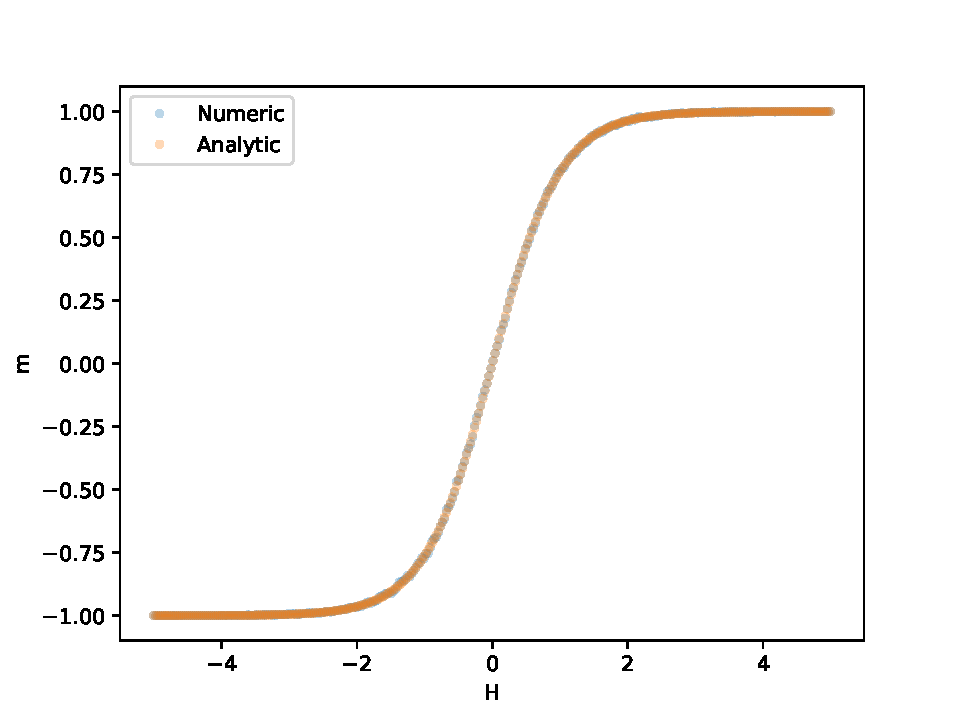
\includegraphics[width=.9\textwidth]{images/Ex1_Graph.pdf}
    \caption{Magnetisierung $m$ in Abhängigkeit des äußeren Magnetfeldes $H$.}
\end{figure}
\begin{figure}
    \centering
    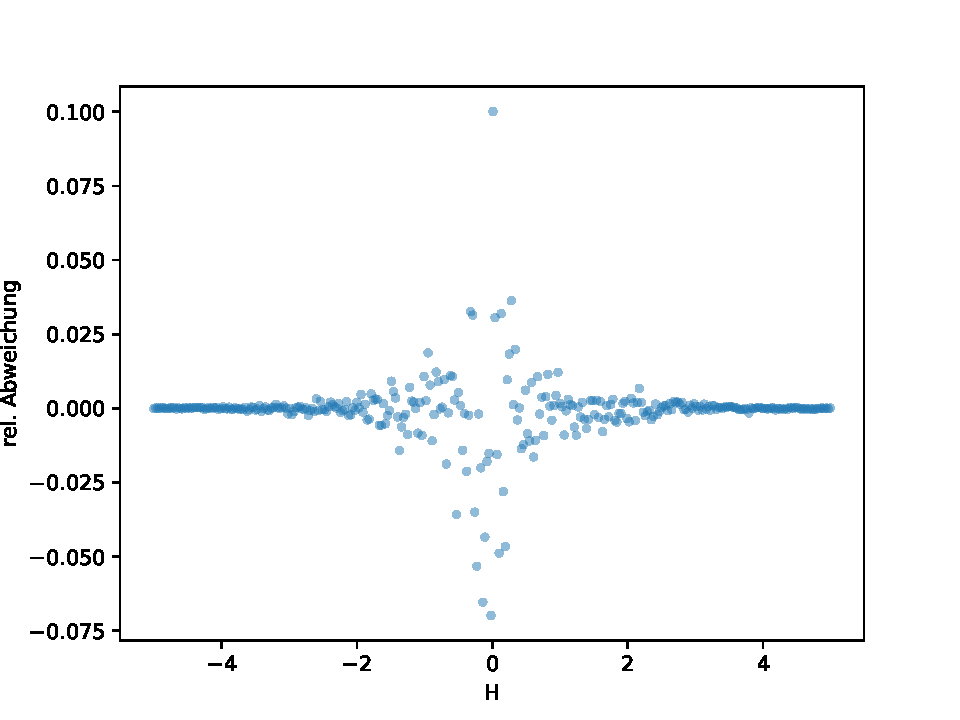
\includegraphics[width=.9\textwidth]{images/Ex1_Abweichung.pdf}
    \caption{Rel. Abweichung zwischen der numerischen und der analytischen Magnetisierung.}
\end{figure}



\subsection{Aufgabe 2} 

\begin{figure}
    \centering
    \begin{subfigure}{0.45\textwidth}
      \centering
      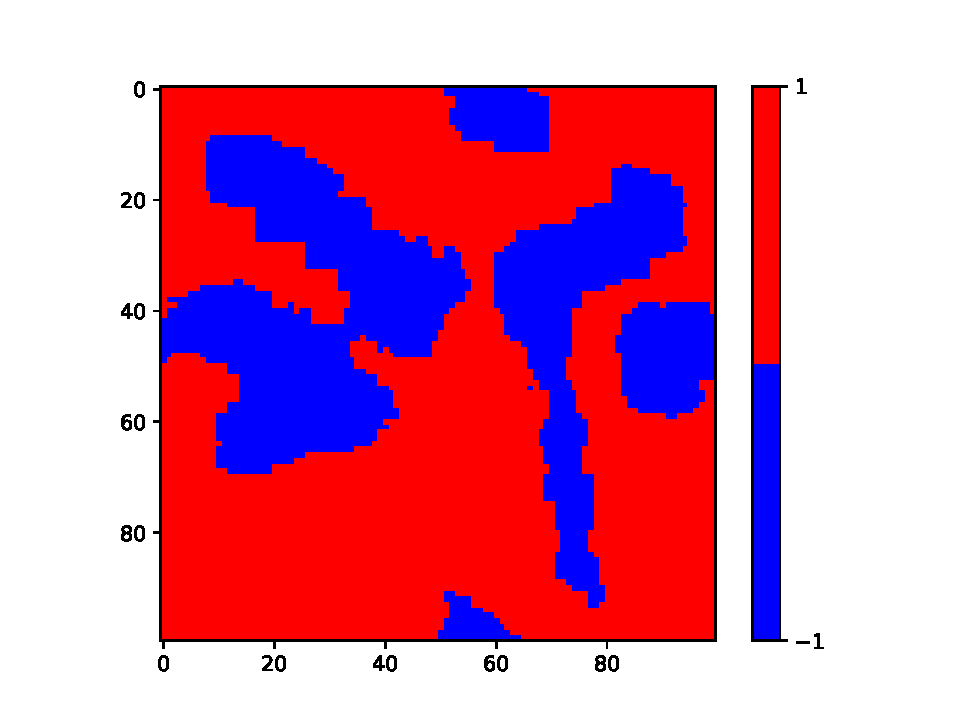
\includegraphics[width=\linewidth]{images/Ising1_0.pdf}
      \caption{Snapshot 1}
      \label{fig:image1}
    \end{subfigure}
    \hfill
    \begin{subfigure}{0.45\textwidth}
      \centering
      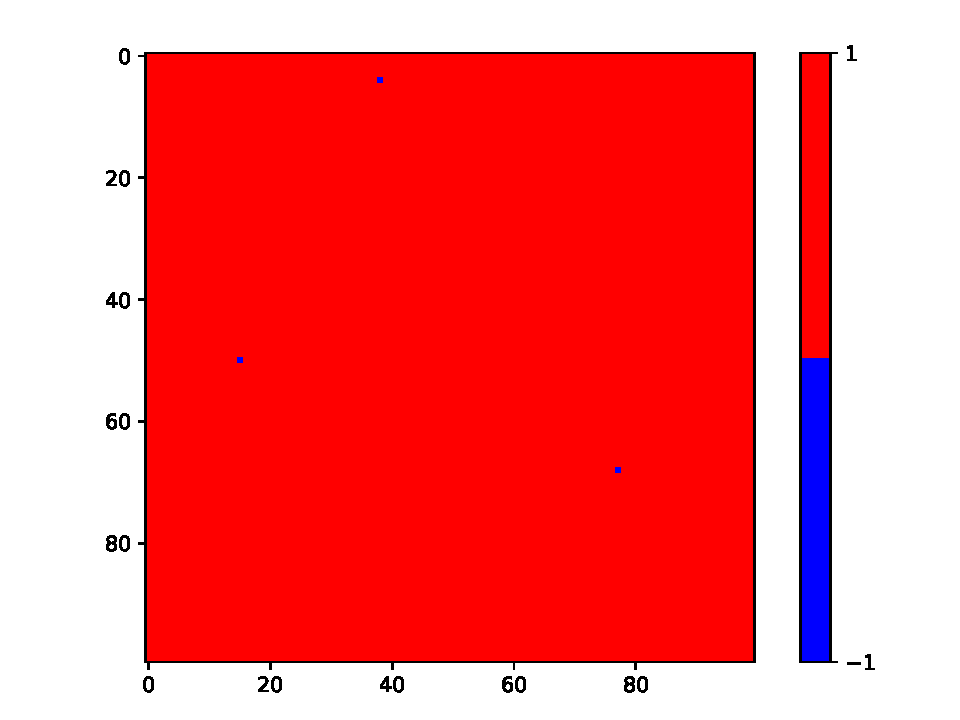
\includegraphics[width=\linewidth]{images/Ising1_2.pdf}
      \caption{Snapshot 2}
      \label{fig:image2}
    \end{subfigure}
    
    \vspace{0.5cm}
    
    \begin{subfigure}{0.45\textwidth}
      \centering
      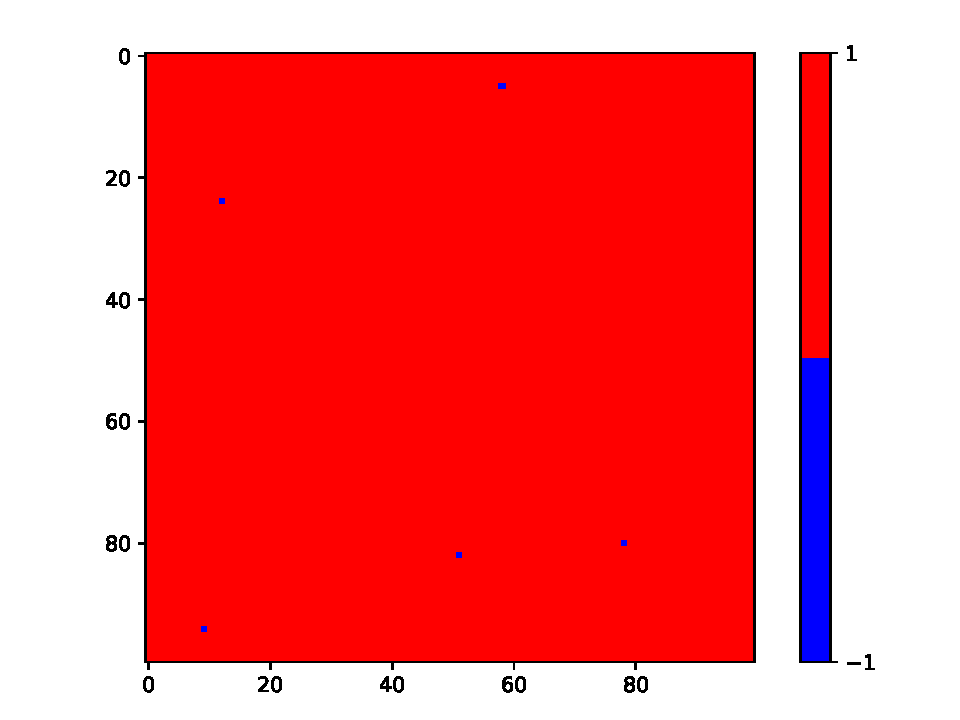
\includegraphics[width=\linewidth]{images/Ising1_3.pdf}
      \caption{Snapshot 3}
      \label{fig:image3}
    \end{subfigure}
    \hfill
    \begin{subfigure}{0.45\textwidth}
      \centering
      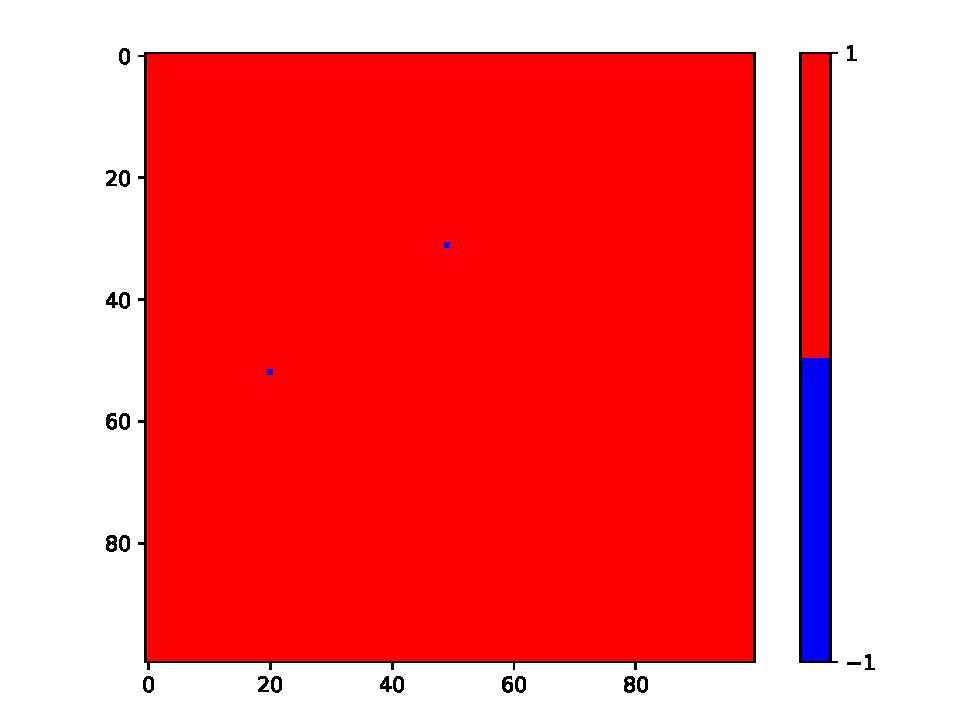
\includegraphics[width=\linewidth]{images/Ising1_4.pdf}
      \caption{Snapshot 4}
      \label{fig:image4}
    \end{subfigure}
    \caption{$k_BT = 1$}
    \label{fig:two_by_two}
  \end{figure}

  \begin{figure}
    \centering
    \begin{subfigure}{0.45\textwidth}
      \centering
      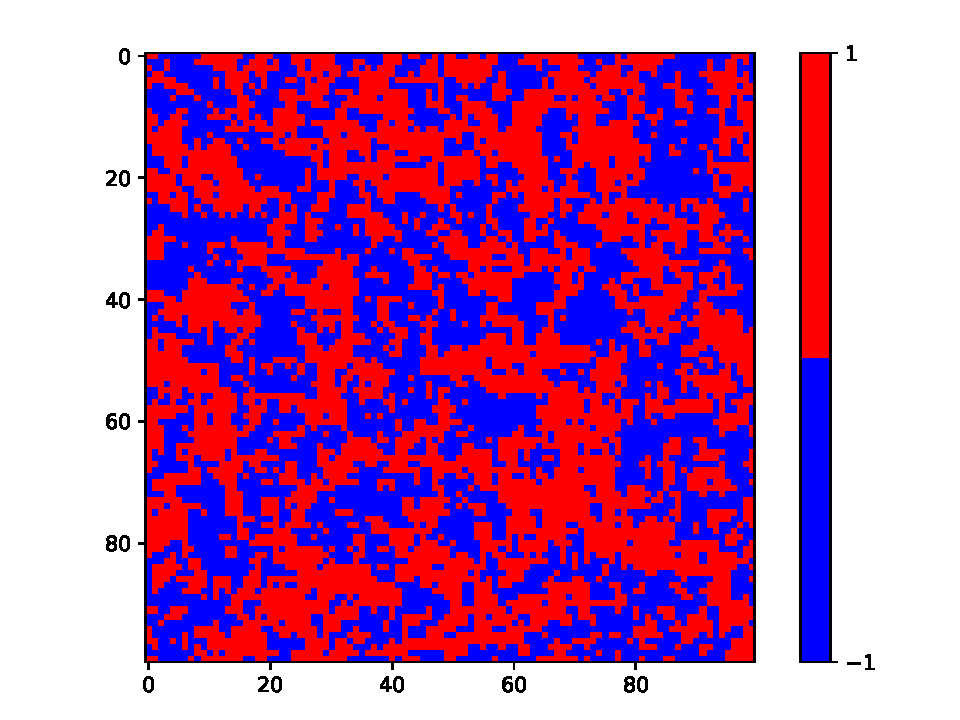
\includegraphics[width=\linewidth]{images/Ising3_0.pdf}
      \caption{Snapshot 1}
      \label{fig:image1}
    \end{subfigure}
    \hfill
    \begin{subfigure}{0.45\textwidth}
      \centering
      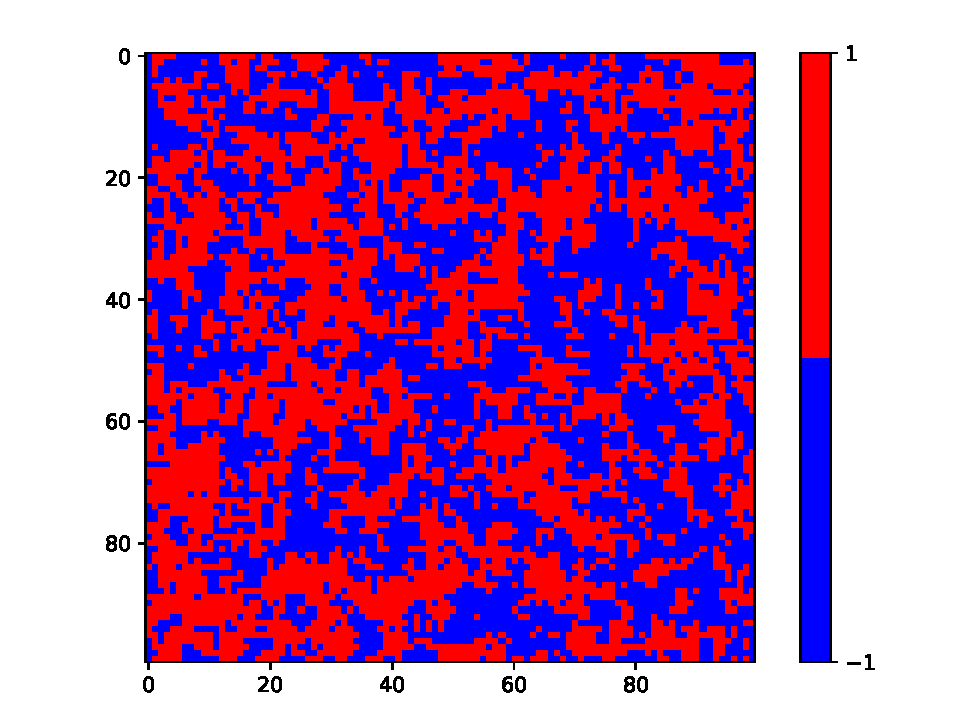
\includegraphics[width=\linewidth]{images/Ising3_2.pdf}
      \caption{Snapshot 2}
      \label{fig:image2}
    \end{subfigure}
    
    \vspace{0.5cm}
    
    \begin{subfigure}{0.45\textwidth}
      \centering
      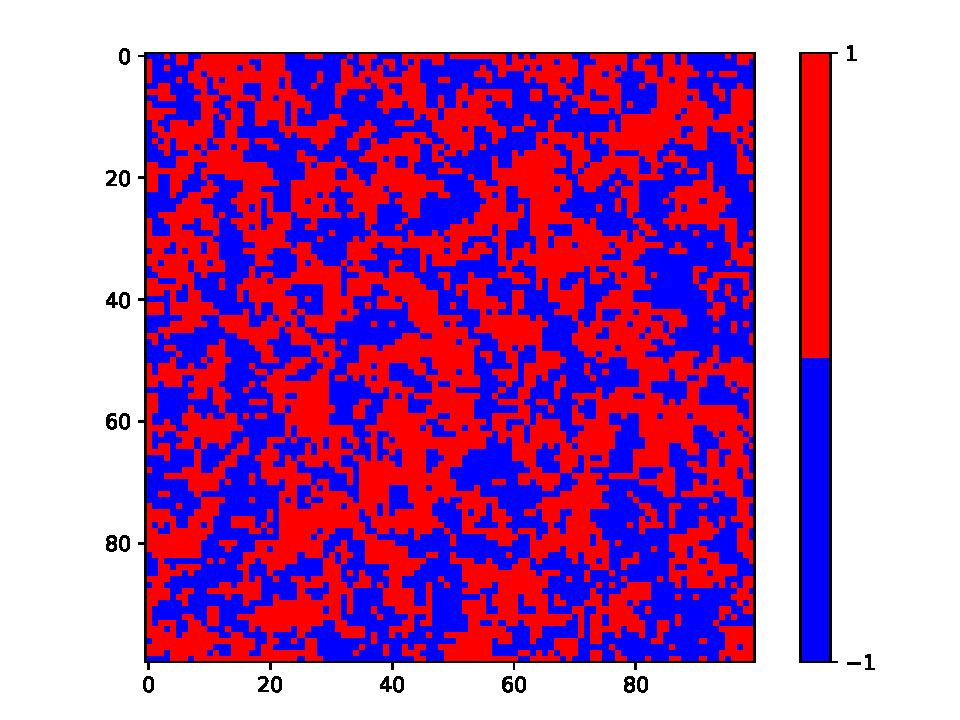
\includegraphics[width=\linewidth]{images/Ising3_3.pdf}
      \caption{Snapshot 3}
      \label{fig:image3}
    \end{subfigure}
    \hfill
    \begin{subfigure}{0.45\textwidth}
      \centering
      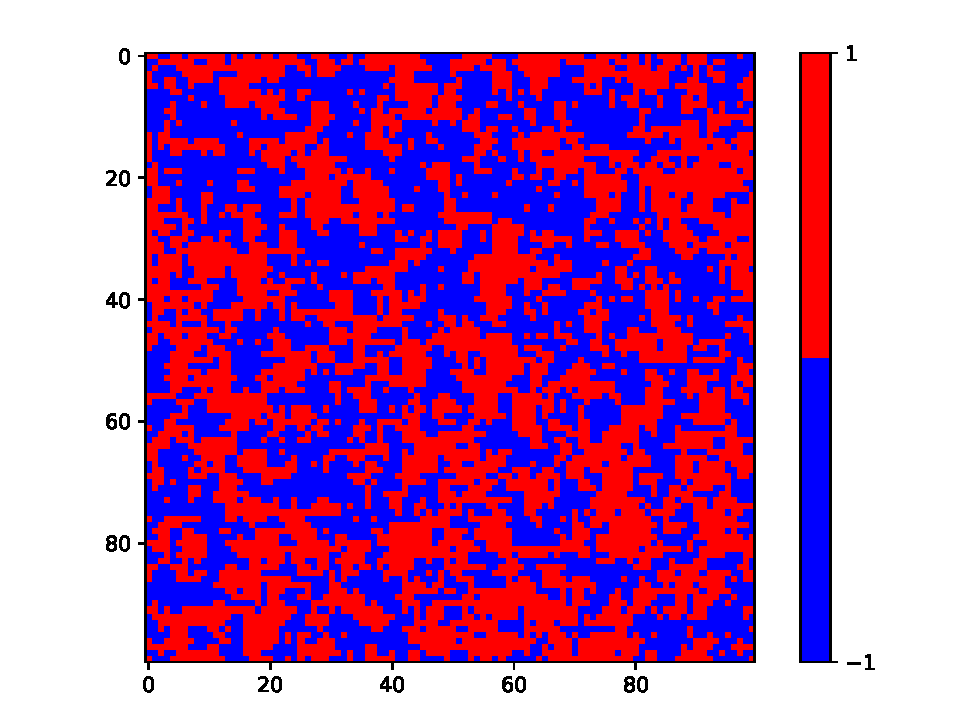
\includegraphics[width=\linewidth]{images/Ising3_4.pdf}
      \caption{Snapshot 4}
      \label{fig:image4}
    \end{subfigure}
    \caption{$k_BT = 3$}
    \label{fig:two_by_two}
  \end{figure}